\documentclass[11pt]{scrartcl}
 \usepackage{tkz-graph} 
 \begin{document} 
 \begin{center} 
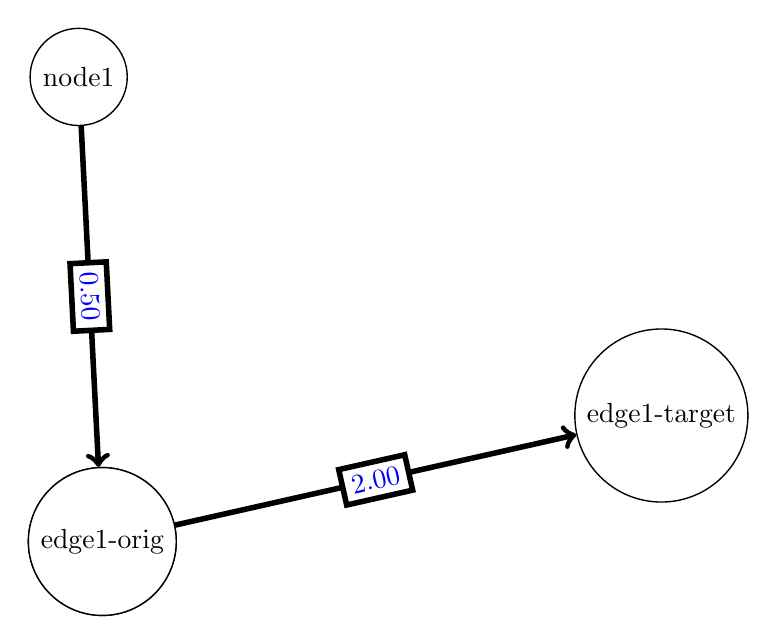
\begin{tikzpicture}  
 \SetVertexNormal[Shape      = circle, FillColor  = orange, LineWidth  = 2pt]
\SetUpEdge[lw  = 2pt,  color      = black,  labelcolor = white,  labeltext  = red, labelstyle = {sloped,draw,text=blue}]
\GraphInit[vstyle=Normal] 
   \SetGraphUnit{10} 
\tikzset{VertexStyle/.append  style={fill}}
\Vertex[x=3.6 ,y=9.7]{edge1-orig}
\tikzset{VertexStyle/.append  style={fill}}
\Vertex[x=10.7 ,y=11.3]{edge1-target}
\tikzset{EdgeStyle/.style={->}}
\Edge[label=$2.00$](edge1-orig)(edge1-target)
\tikzset{VertexStyle/.append  style={fill}}
\Vertex[x=3.3 ,y=15.6]{node1}
\tikzset{VertexStyle/.append  style={fill}}
\Vertex[x=3.6 ,y=9.7]{edge1-orig}
\tikzset{EdgeStyle/.style={->}}
\Edge[label=$0.50$](node1)(edge1-orig)
\end{tikzpicture}
 \end{center}  
 \end{document}

